\documentclass{report}
\usepackage{amsmath} 
\usepackage{amstext}
\usepackage{amssymb} 
\usepackage[latin1]{inputenc}
%\usepackage{nomencl}
\usepackage{setspace}
\usepackage{color}
\usepackage{graphicx}       % EPS figures
\usepackage{varioref}       % smart page, figure, table, and equation

\usepackage[tight]{subfigure}      % subcaptions for subfigures
%\usepackage[pdftex]{graphicx}
\usepackage[colorlinks]{hyperref} 
%\DeclareGraphicsExtensions{.pdf,.png,.jpg}
%
% Define contents of the title
%
\title{A Surface Blocking Tutorial For Generating Geometry for pyGeo}

\author{Gaetan Kenway}


\usepackage{qresize}
\setlength{\textwidth}{7in}
\setlength{\textheight}{10in}
\resize  


%%%%%%%%%%%%%%%%%%%%%%%%%%%%%%%%%%%%%%%%%%%%%%%%%%%%%%%%%%%%%%%%%%%%%
% BEGIN OF DOCUMENT
%%%%%%%%%%%%%%%%%%%%%%%%%%%%%%%%%%%%%%%%%%%%%%%%%%%%%%%%%%%%%%%%%%%%%
\begin{document}
%
% Generates the title of the document
\maketitle


\section{Introduction}

This is a tutorial which shows how to generate a structured surface grid using ICEMCFD which can be used as input to the pyGeo framework. The particular example we will be working with is a generic sort of wing-body geometry. The fundamentals of surfacing blocking generation should carry over to more complex geometries.

\section{Geometry Generation}

The first step is to generate the two geometries we wish to use. 


\subsection{Wing}

The wing can be generated directly from pyGeo. The steps to generate the wing geometry are as follows:

\begin{itemize}
\item Locate the gen\_wing\_iges.py in the root directory of this tutorial.
\item A quick look at the file will reveal this will generate a two section swept, twisted wing with a slight amount of dihedral. 
\item The ``writeIGES'' command at the bottom of the script writes the iges file to disk.
\end{itemize}

\subsection{Fuselage}

The fuselage is provided as a iges file. It was originally generated in SolidWorks and the original Solid Works 2008 file is included for reference as ``fuse.sldprt''

\subsection{Geometry Importing into ICEMCFD}

Once we have the two iges files, we start ICEM and click: \\
\begin{itemize}
\item File -$>$ Import Geometry -$>$ STEP/IGES
\end{itemize}
Select the wing.iges which was generated above. Leave the default iges load options. Don't save the project yet, we will do that after we add the fuselage.

Next, do the same sequence again and add the fuse.iges file. When prompted, select Merge geometries.

Now, you should see something like figure~\ref{fig:geo_load}.

\begin{figure}[htb]
 \centering
 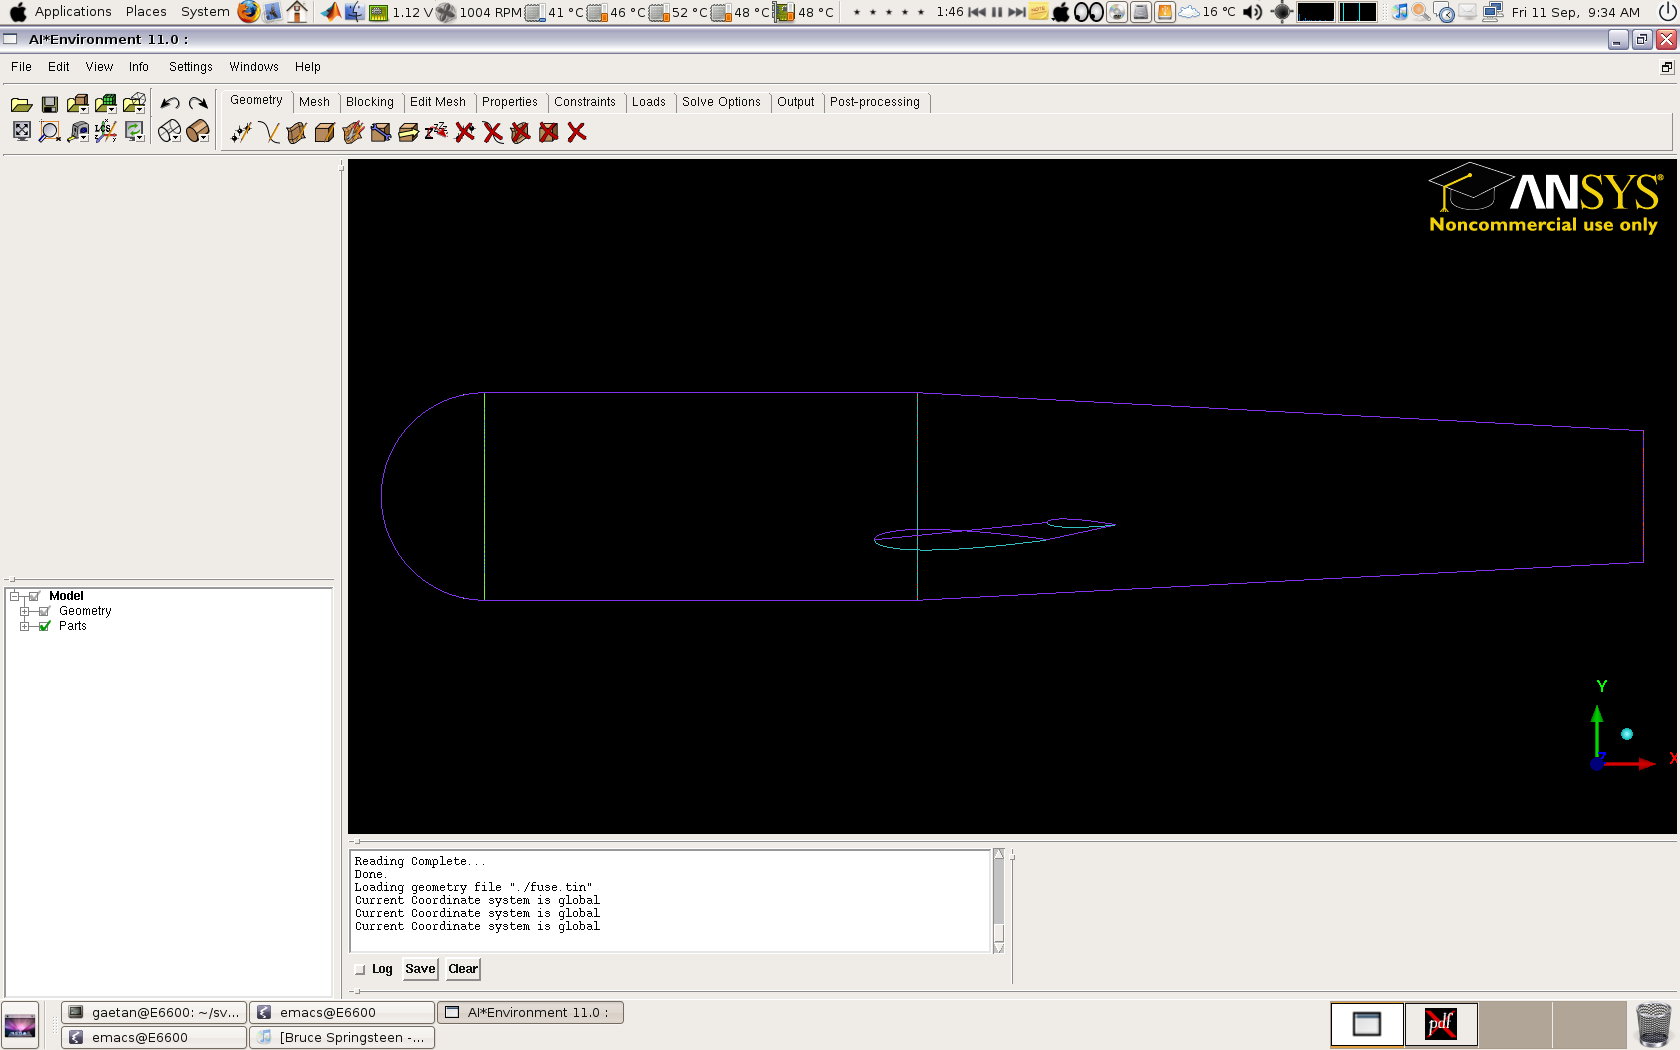
\includegraphics[width=\textwidth,angle=0]{figures/fig1.png}
 \caption{fig:geometry after loading}
 \label{fig:geo_load}
\end{figure}

Now you can save the project.

\section{Geometry Modification}

Before we can start the surface blocking procedure, we need to do some geometric modifications to the geometry we just imported. Specifically we will do the following steps:

\begin{enumerate}
\item Remove the face on the mirror plane belonging to the fuselage.
\item Intersection the fuselage with the wing to produce the intersection curves
\item Remove the section of the wing surface that is now hidden inside the fuselage
\item Produce curves on the fuselage surface which form the edges of our final surface blocks
\end{enumerate}

\subsection{Face Removal}
Under the geometry tab select the ``Delete Surface'' button. Click on the flat surface that is on the mirror plane (with the left mouse button) and then confirm your selection with the middle button. This left-mouse to select, and middle to confirm is used extensively in ICEM.

Now after rotating the geometry, clicking on the ``Surfaces'' in the geometry list and setting the display mode to ``Solid Full Display'' we should have something that looks like figure~\ref{fig:geo_surface_removed}

\begin{figure}[htb]
  \centering
  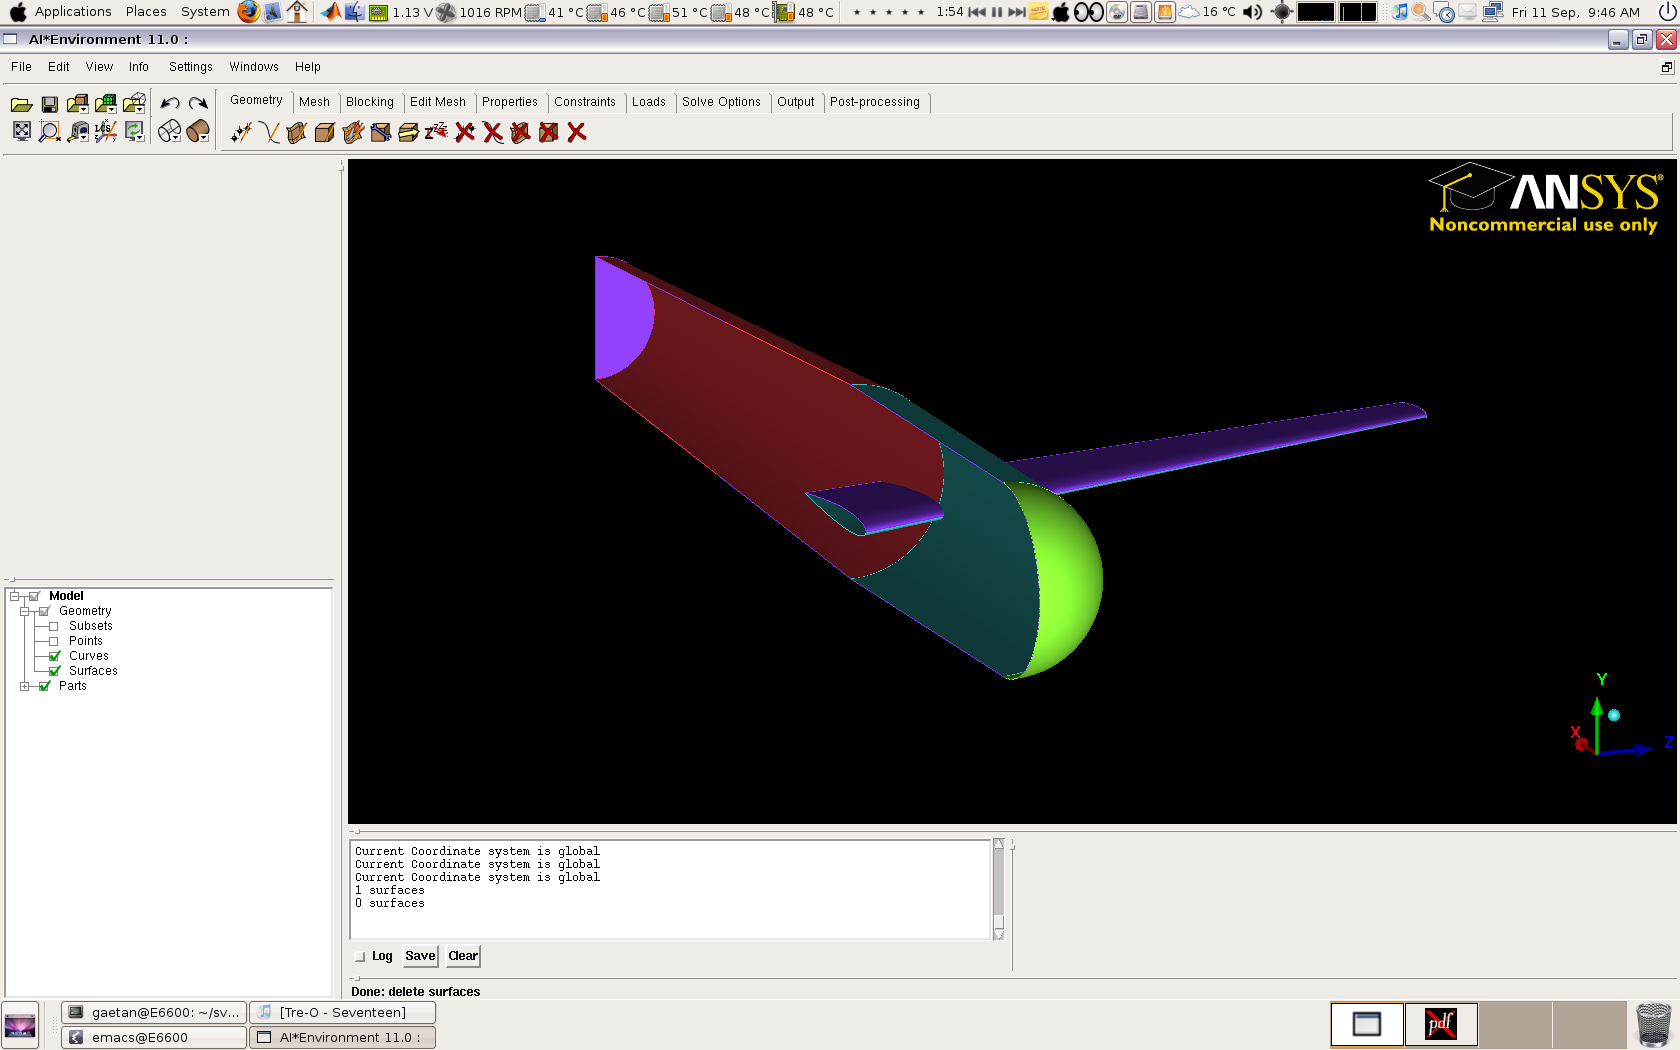
\includegraphics[width=\textwidth,angle=0]{figures/fig2.png}
  \caption{Geometry after mirror plane surface removed}
  \label{fig:geo_surface_removed}
\end{figure}

\subsection{Surface Intersection}

The next step is to perform the surface intersections. Thankfully this isn't difficult. Under the Geometry Tab click on ``Curve'' button and then on the ``Surface Intersection''. In this case there are actually 4 surfaces we need to intersection: Two on the fuselage and two on the wing. Using the left mouse select the upper wing surface and ONE of the two it intersects on the fuselage. ONE new curve should show up. Then repeat this for the other 3 combinations: Upper surface other fuse patch and two for the lower surface.  figure~\ref{fig:intersection_curve}
\begin{figure}[htb]
  \centering
  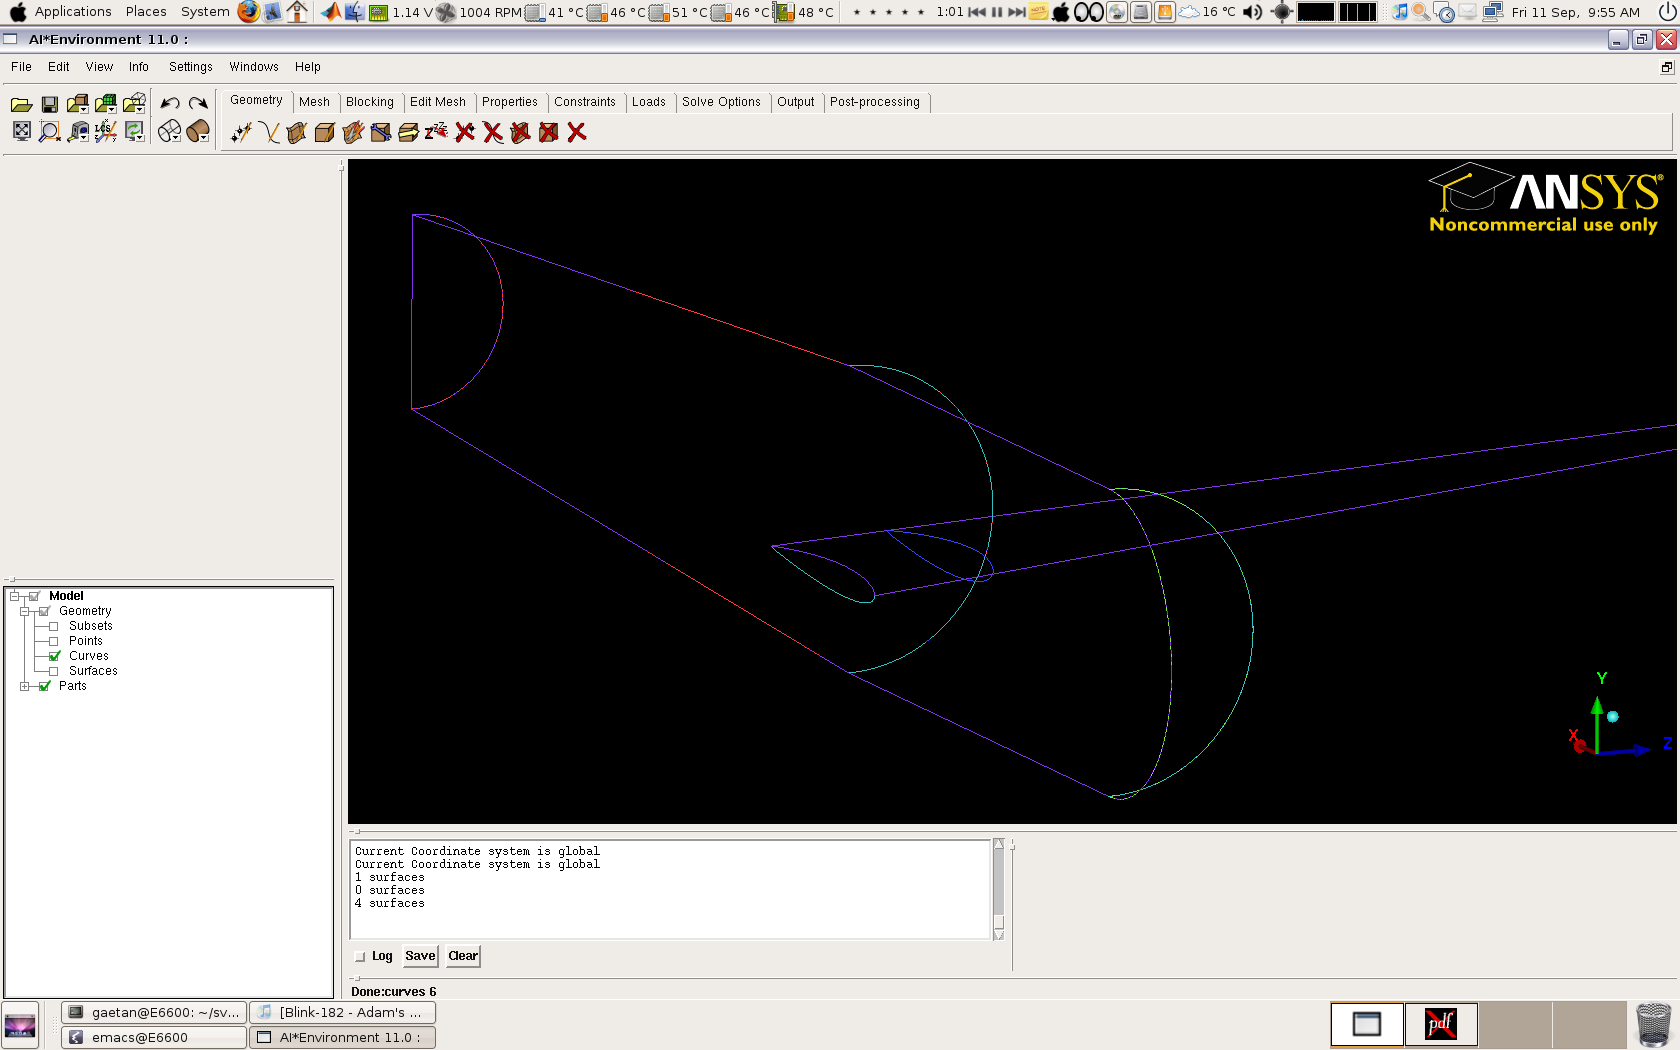
\includegraphics[width=\textwidth,angle=0]{figures/fig3.png}
  \caption{Geometry after intersection curve generated. The new intersection curve is the blue one.}
  \label{fig:intersection_curve}
\end{figure}

\subsection{Interior Face Removal}

Now we want to remove the surfaces interior to the fuselage. However before we can do this, we must ``Split'' the wing surfaces at the intersection curves that were created in the previous step. Under ``Geometry'' click ``Create/Modify Surfaces'' and then click ``Segment Trim Surface''. Make sure the method is ``By Curve''. You should see two selection boxes, one for the surfaces to trim and the other for the curves. Select the two surfaces with the left/middle combo as described above. Then select ALL 4 intersection curve that were created previously.

We should get a bunch more curves and surfaces. Now, using the ``remove curve'' and ``remove surface'' commands select all the geometry that is internal to the fuselage to remove it.

After this clean-up we should have a fairly clean geometry that looks like figure~\ref{fig:cleaned_up_geo}
\begin{figure}[htb]
  \centering
  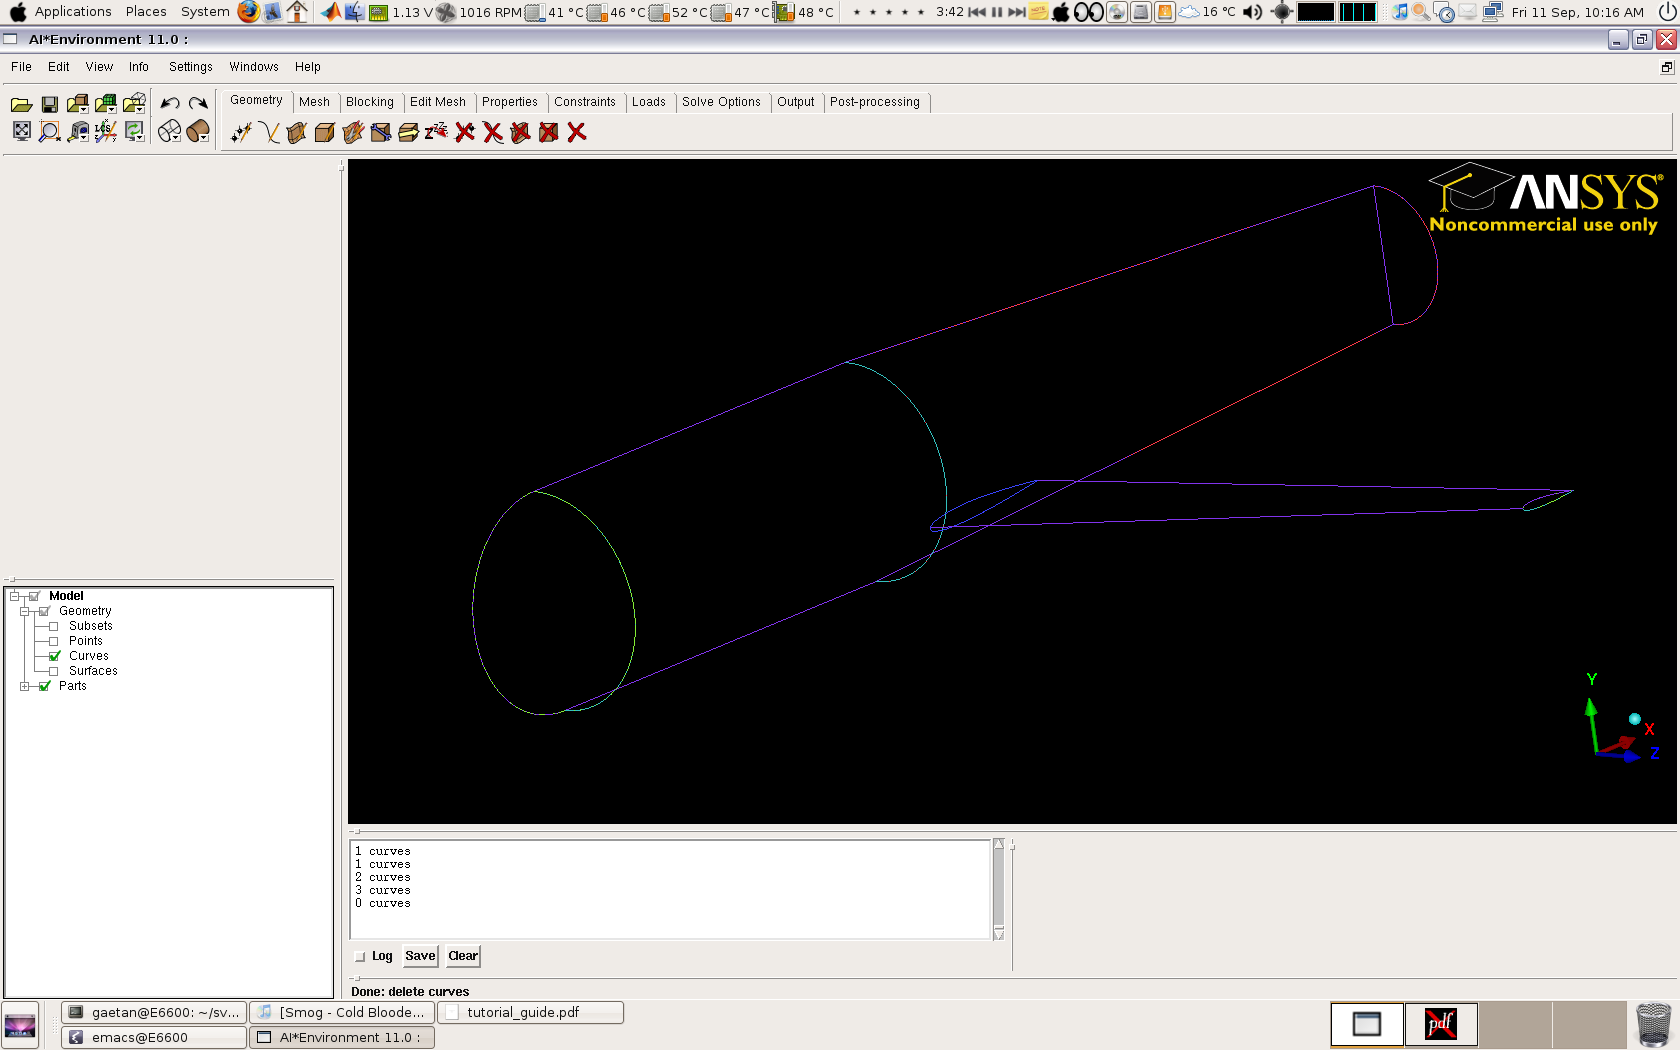
\includegraphics[width=\textwidth,angle=0]{figures/fig4.png}
  \caption{Geometry after split surface geometry cleaned up}
  \label{fig:cleaned_up_geo}
\end{figure}

\subsection{Surface Blocking Edges}
The last geometry modification step is to generate the curve on the surface where we will eventually attach the edges of the surface blocks.  We need to make 10 lines as follows:

\begin{itemize}
\item Leading edge of wing to fuselage nose
\item Trailing edge of wing to middle of tail arc
\item Leading edge vertically to upper surface of fuselage
\item Leading edge vertically to lower surface of fuselage
\item Middle of upper surface of wing to upper surface of fuselage
\item Middle of lower surface of wing to lower surface of fuselage
\item Trailing edge of wing to upper surface of fuselage
\item Trailing edge of wing to lower surface of fuselage
\item Middle of upper surface root to middle of upper surface tip
\item Middle of lower surface root to middle of lower surface tip
\end{itemize}

Now make sure the ``points'' in geometry are turned on. You may see some spurious points which can be deleted. The procedure for making a curve on the surface is to make a straight line and then ``project'' it onto the surface. We will first make the points at the places where we want the edges to connect. 

Make points at the following places:

\begin{itemize}
\item Nose
\item Point on upper fuselage curve approximately above leading edge
\item Point on lower fuselage curve approximately below leading edge
\item Point on upper fuselage curve approximately above middle of upper wing surface
\item Point on lower fuselage curve approximately below middle of lower wing surface
\item Point on upper fuselage curve approximately above trailing edge
\item Point on lower fuselage curve approximately below trailing edge
\item Point on middle of tail section arc
\item Point on middle of tail section on mirror plane
\item Point on upper middle of wing root 
\item Point on lower middle of wing root
\item Point on upper middle of wing tip
\item Point on lower middle of wing tip
\end{itemize}

To create points on the screen click ``Create Points'' in the ``Geometry'' tab and then the ``Screen Select'' button.

You should have points in approximately the places shown in figure~\ref{fig:points}

\begin{figure}[htb]
  \centering
  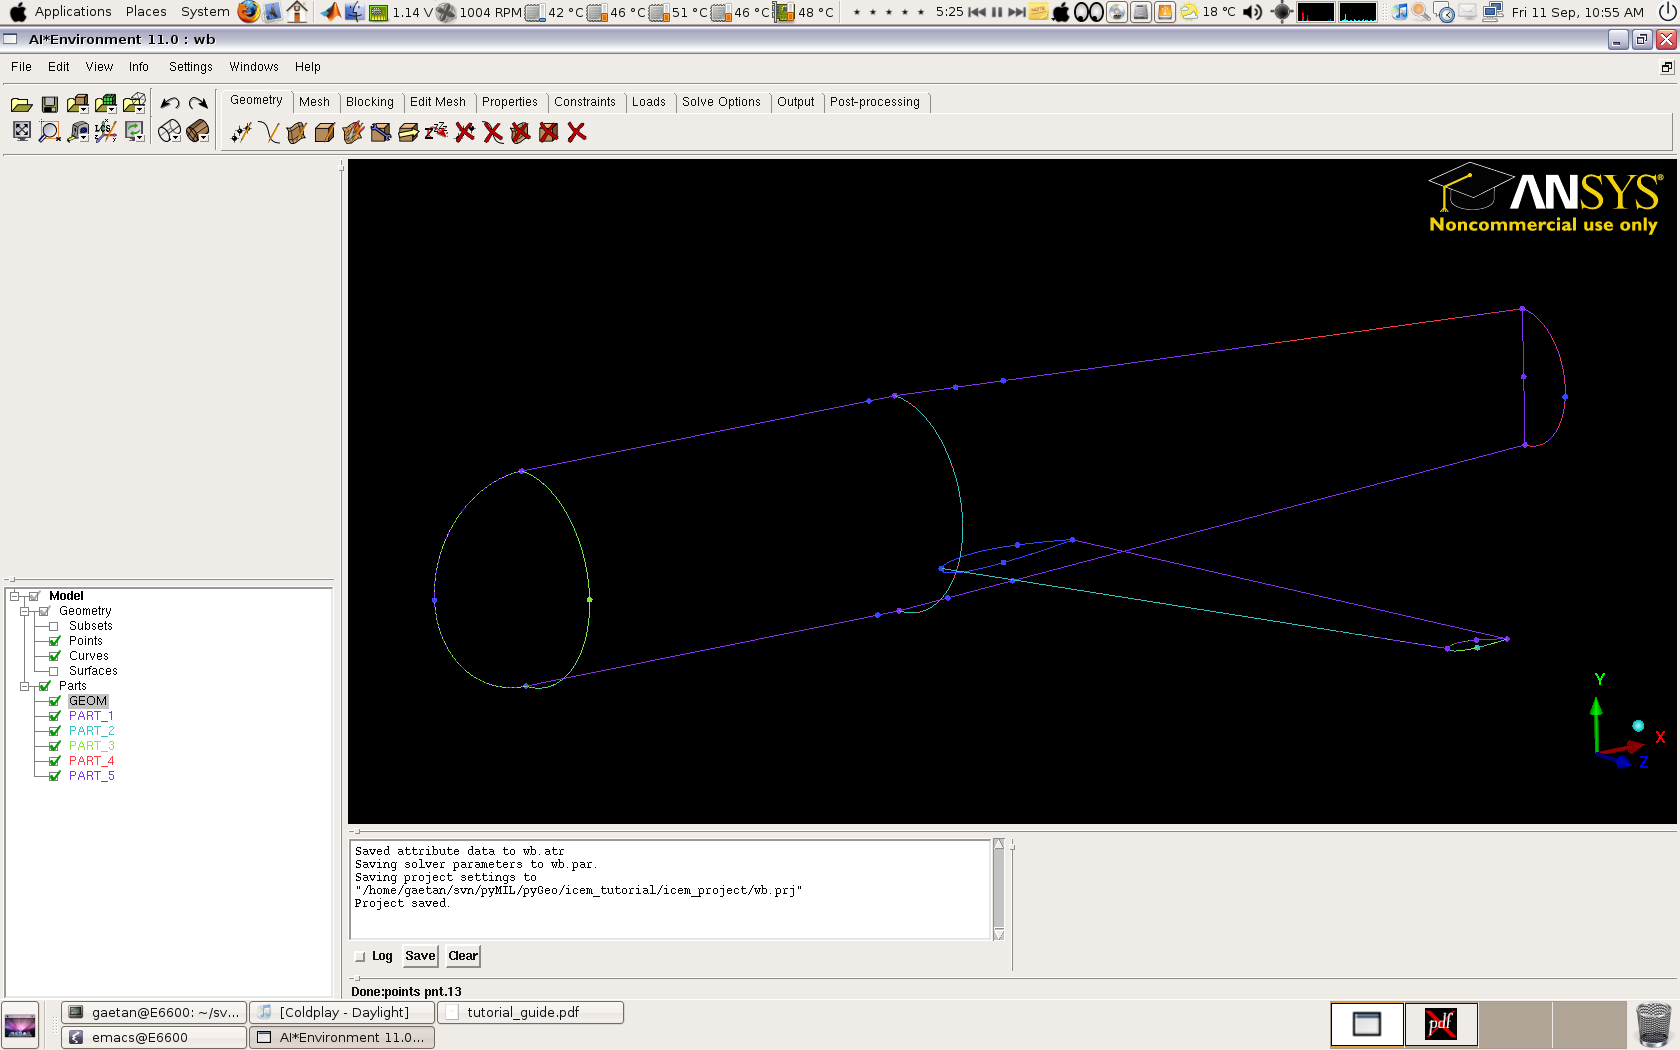
\includegraphics[width=\textwidth,angle=0]{figures/fig5.png}
  \caption{Points on curves}
  \label{fig:points}
\end{figure}

Now, using under ``Geometry'' click ``Create Modify Curve'' and the first button ``From Points''. Create the lines described above using the points we just created.

Now you should have straight lines that look like figure~\ref{fig:lines}

\begin{figure}[htb]
  \centering
  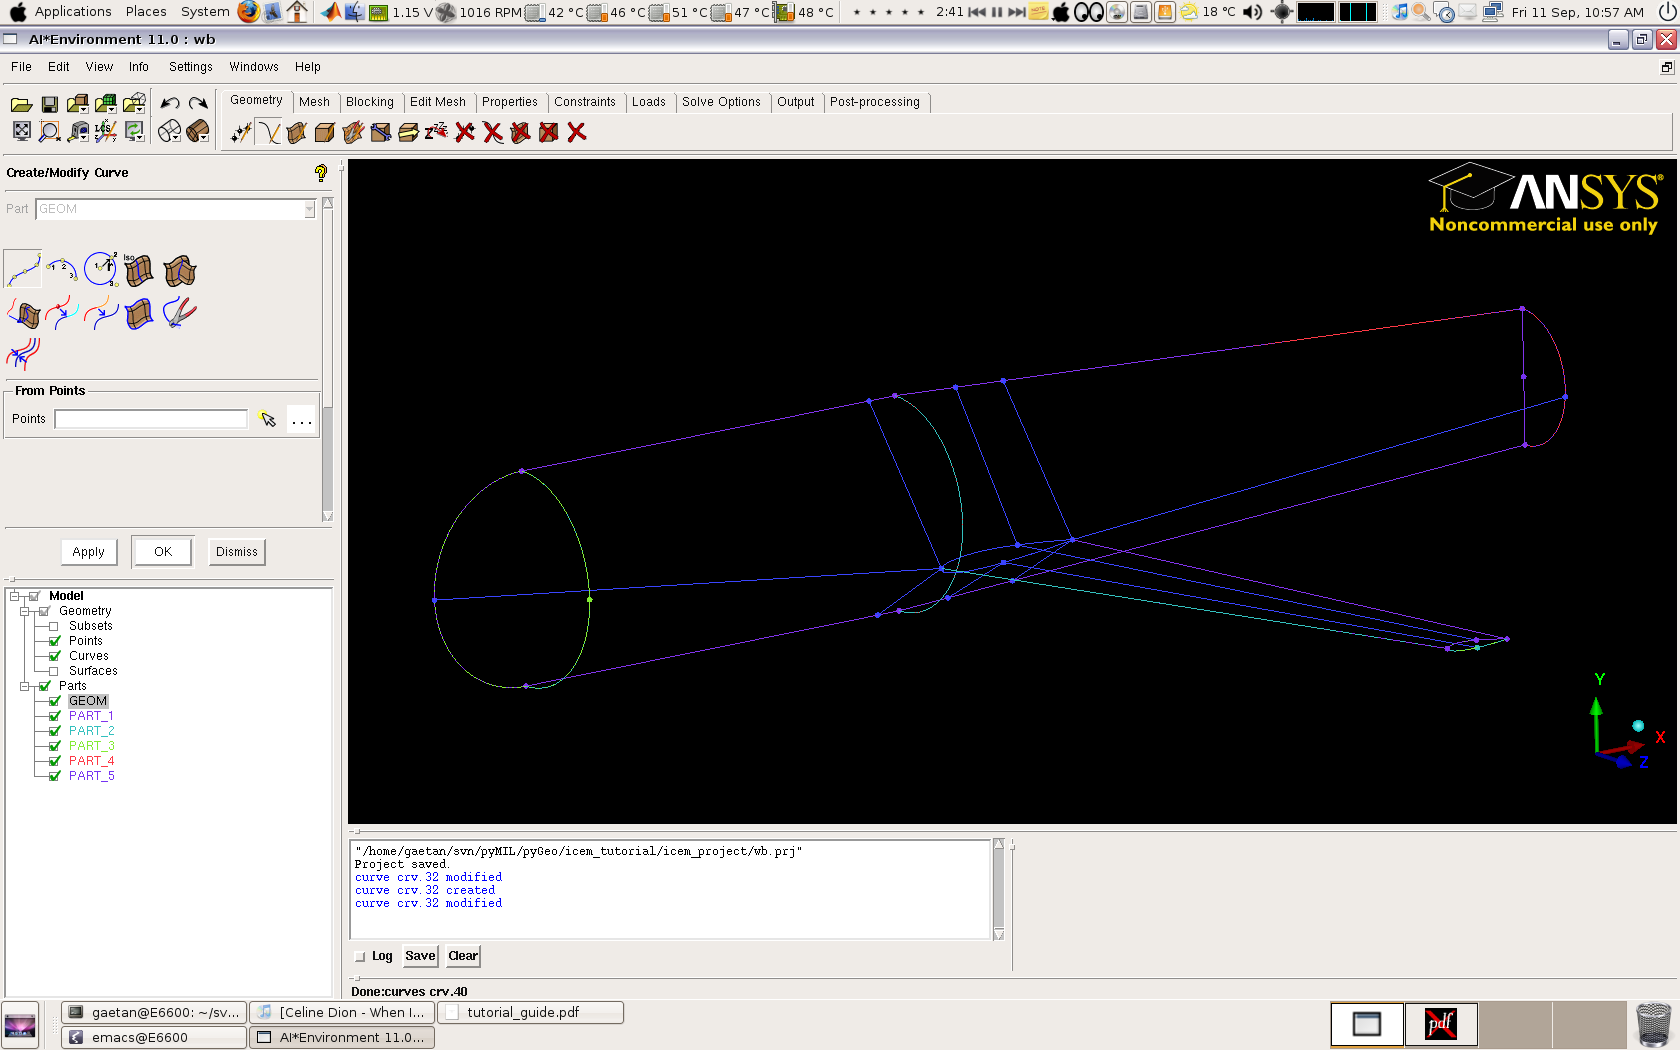
\includegraphics[width=\textwidth,angle=0]{figures/fig6.png}
  \caption{Lines before projection}
  \label{fig:lines}
\end{figure}

Now we will project the lines onto the respective surfaces. Again under ``Geometry'', ``Create/Modify Curve'' click ``Project Curve on Surface''. The default method is ``Normal to Surface''. For the fuselage projections, we want to change that to ``Specify Direction''. Then scroll down and select ``Z -Direction'' under the direction option.
For the two on the wing surface, select the ``Normal to Surface'' option. Select the curve you are projecting and the surfaces it crosses, and then the middle button to make the projected curves. 

Usually, I delete the unprojected curves after they are projected since it keeps a less cluttered geometry. You should now get a geometry that looks like figure~\ref{fig:projected_lines}

\begin{figure}[htb]
  \centering
  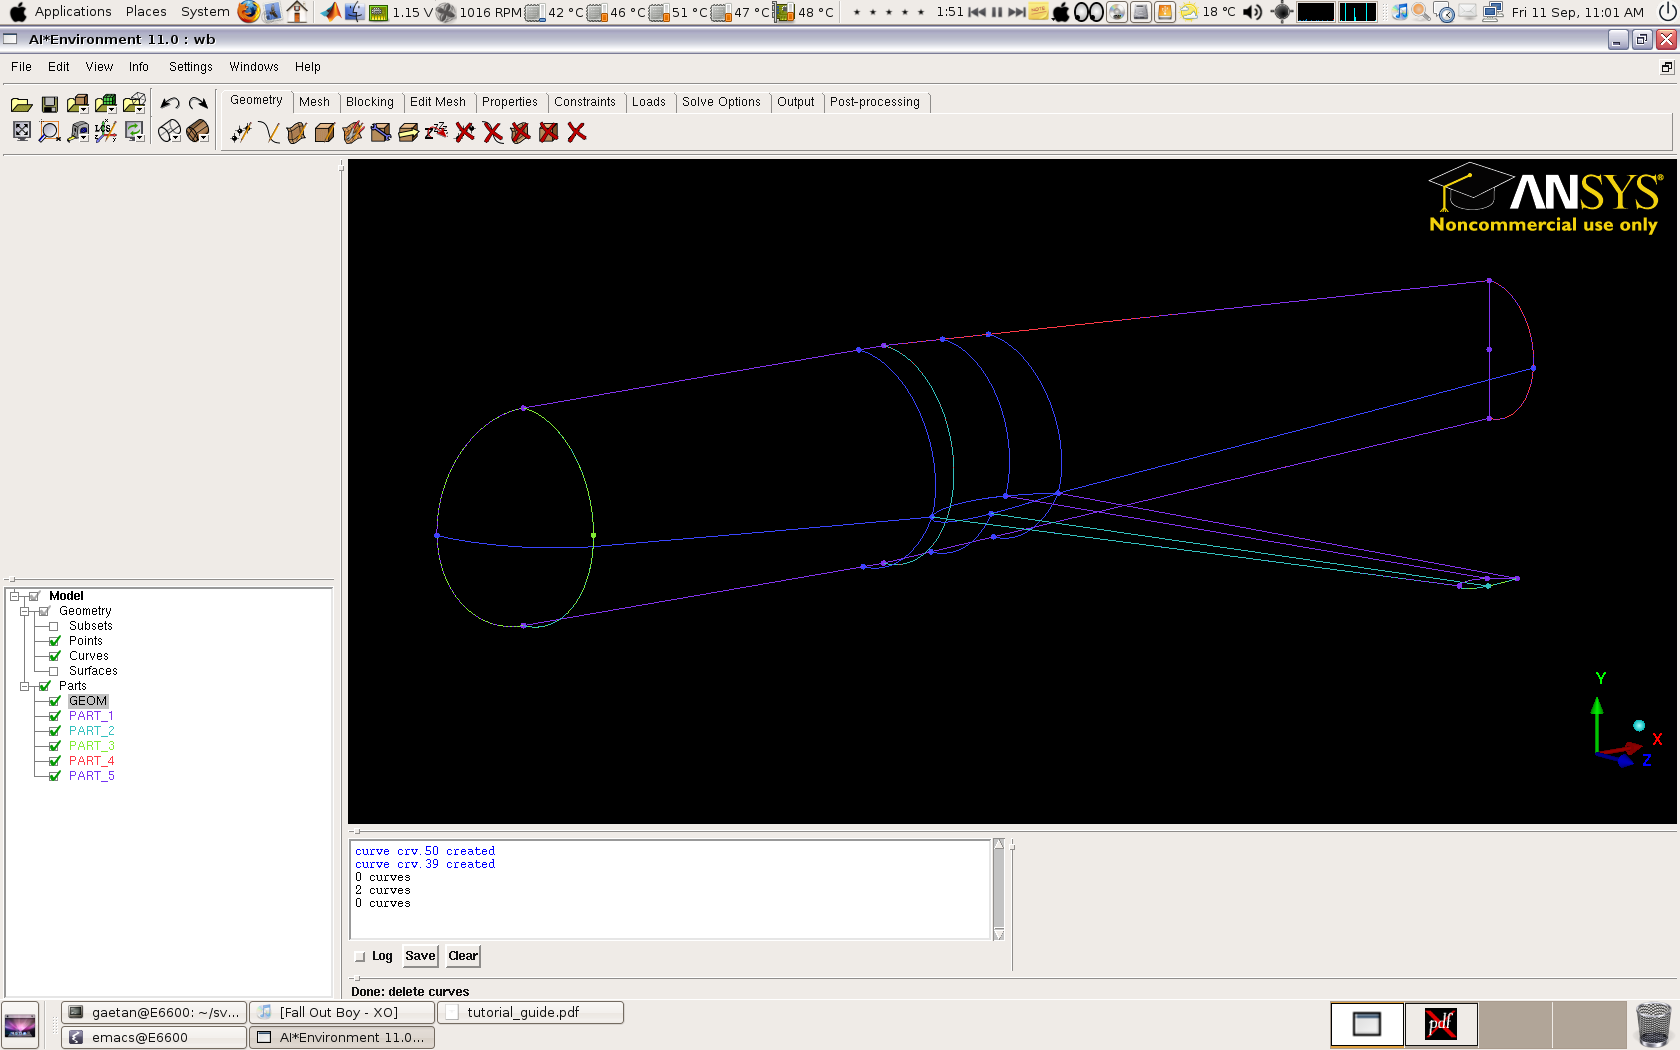
\includegraphics[width=\textwidth,angle=0]{figures/fig7.png}
  \caption{Lines after projection}
  \label{fig:projected_lines}
\end{figure}

Now we are ready to do the surface blocking!

\section{Surface Blocking}

By now it should be clear how the geometry will be divided into blocks. Briefly, we will have two (degenerate) surface in front of the wing, two patches on top of the wing, two below the wing, two behind the wing, two degenerate patches on the wing tip and two degenerate patches on the rear surface.

Now go to the ``Blocking'' tab and click the ``Create Block'' button. ICEM is supposed to do some blocking automatically but it never does what it should and is generally useless. However, we must use the create new blocking function to start blocking. Under type select ``2D Surface Blocking'' , ``Mostly Mapped'', select ``All Quad'' for ``2D Mesh Type'' option. Finally select the surface button and select 1 surface. It doesn't really matter, since we will immediately delete this block. Take the upper surface of the wing for example. 

If we turn off all the geometry and under blocking just have ``edges'' clicked you should see something like figure~\ref{fig:init_block}.
\begin{figure}[htb]
  \centering
  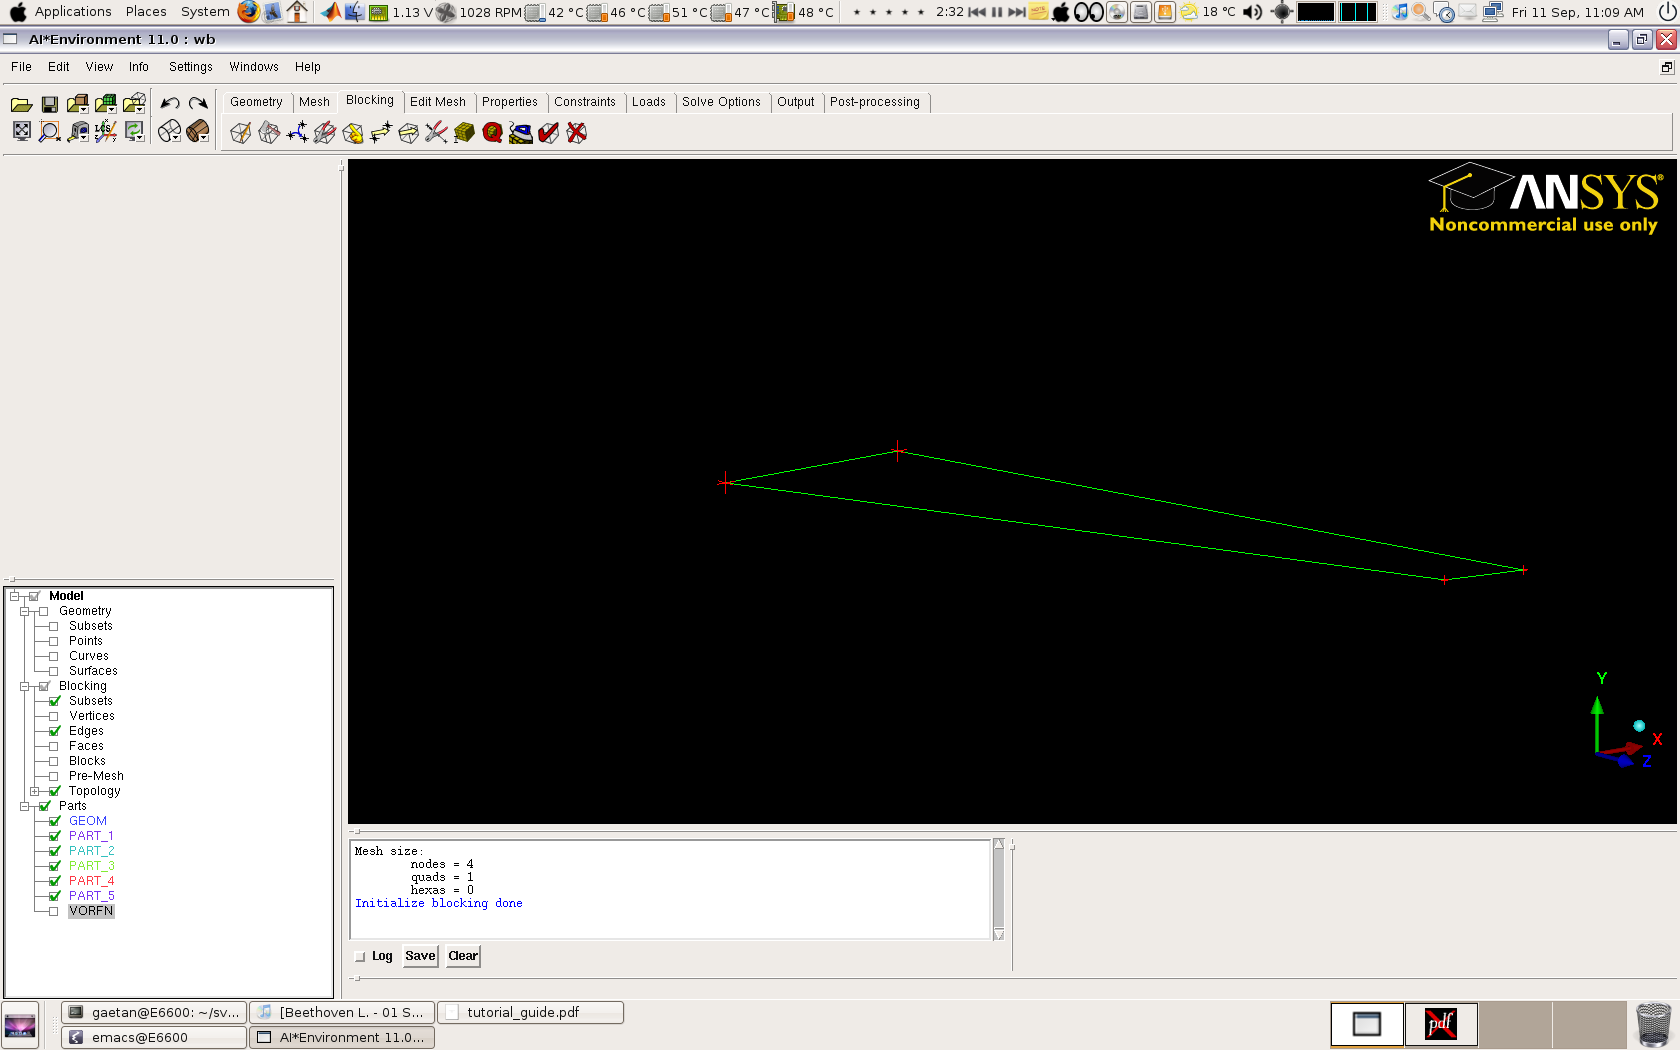
\includegraphics[width=\textwidth,angle=0]{figures/fig8.png}
  \caption{Initial Block}
  \label{fig:init_block}
\end{figure}

Click on the ``Delete Block'' button and delete the block.

Now we are ready to add our own blocks. Surface block are added with FOUR nodes. Even if you want a degenerate block you must STILL start it with FOUR nodes and then merge then. Got that MUST HAVE FOUR (4) NODES! Now create the blocks using the points we created earlier. 

Select the ``New Block'' command and then the second one ``From Vertices''

Select the 4 vertices containing the surface patch above the forward section of the wing. 

A Note on selecting nodes: When you are selecting vertices it tries to select the ``vertex'' type first. These are the logical block vertices.  YOU MUST SELECT THESE FIRST if they exist. THEN click the middle button and you select the rest using regular geometry points. Verticies are NOT selected in a CW or CCW ordering. You select two points along the first parametric direction (u) and then the other two in the same direction. Example if If you have a unit square from (0,0) to (1,1) an example of the point select order is (0,0),(1,0),(0,1),(1,1). That will orient the u axis along x and the v axis along y.

The first four blocks on the fuselage on top and below the wing (with geometry turned off) looks like figure~\ref{fig:four_blocks}.
\begin{figure}[htb]
  \centering
  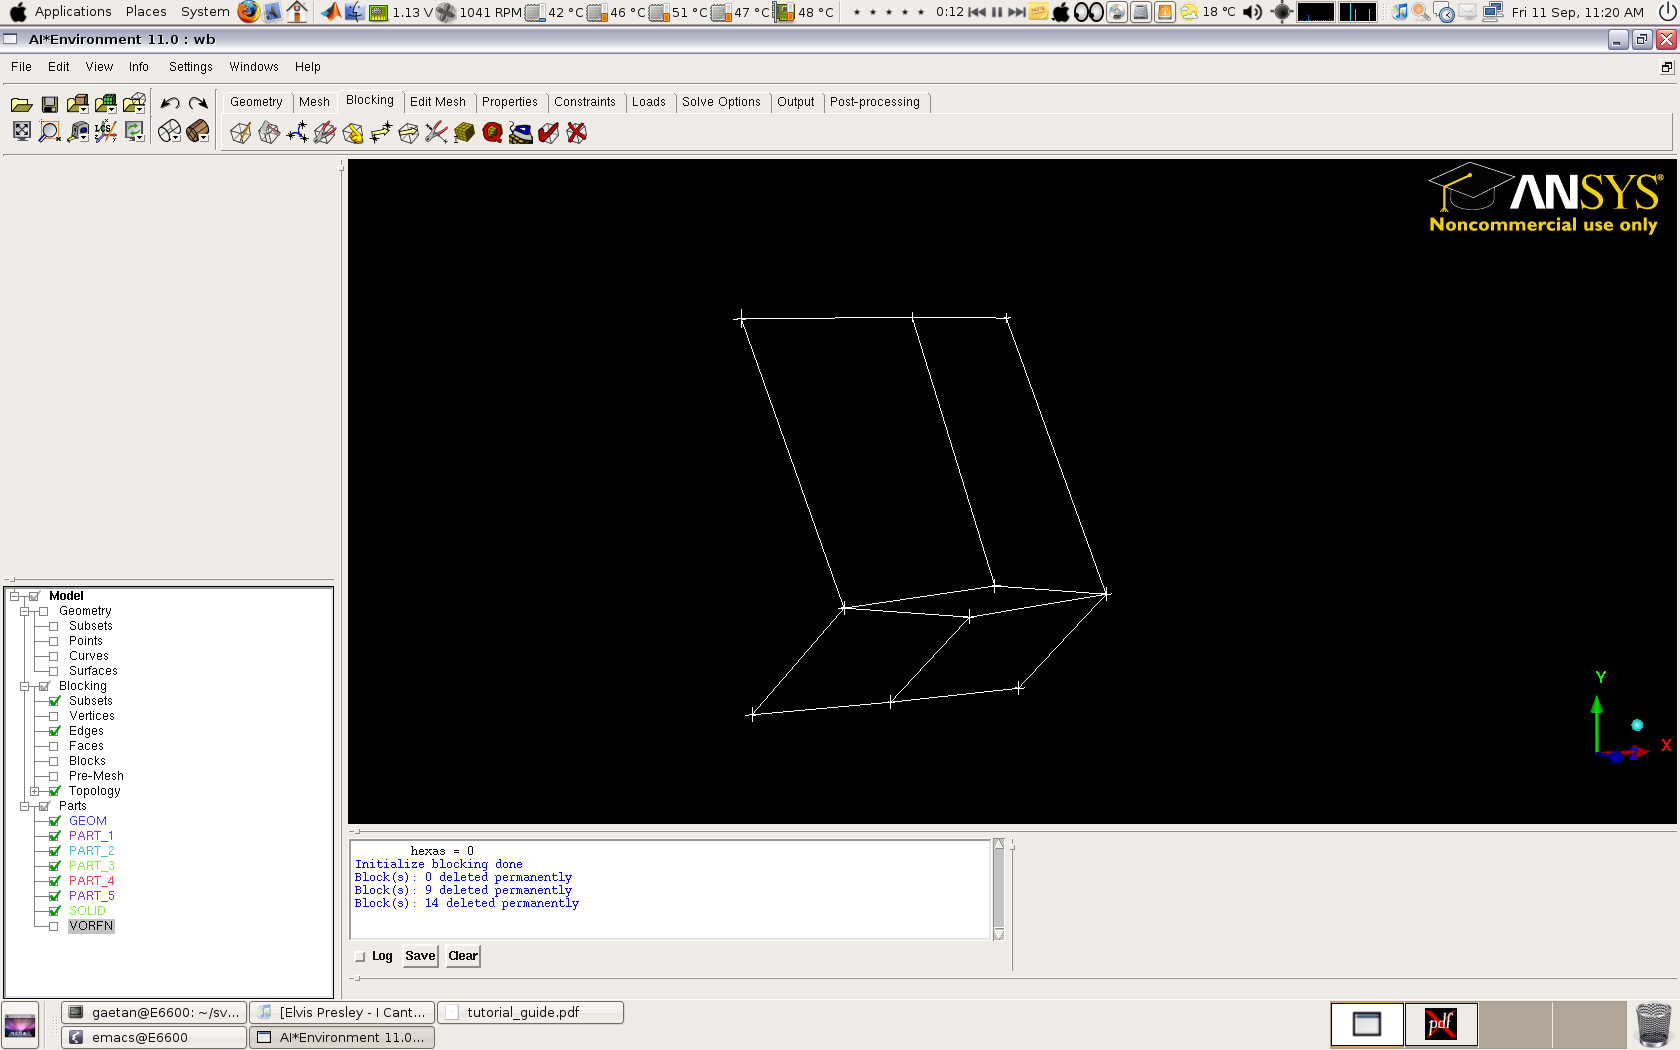
\includegraphics[width=\textwidth,angle=0]{figures/fig9.png}
  \caption{First four blocks}
  \label{fig:four_blocks}
\end{figure}


Now add the four blocks on the wing surface, and the two behind the wing to generate figure~\ref{fig:more_blocks}.

\begin{figure}[htb]
  \centering
  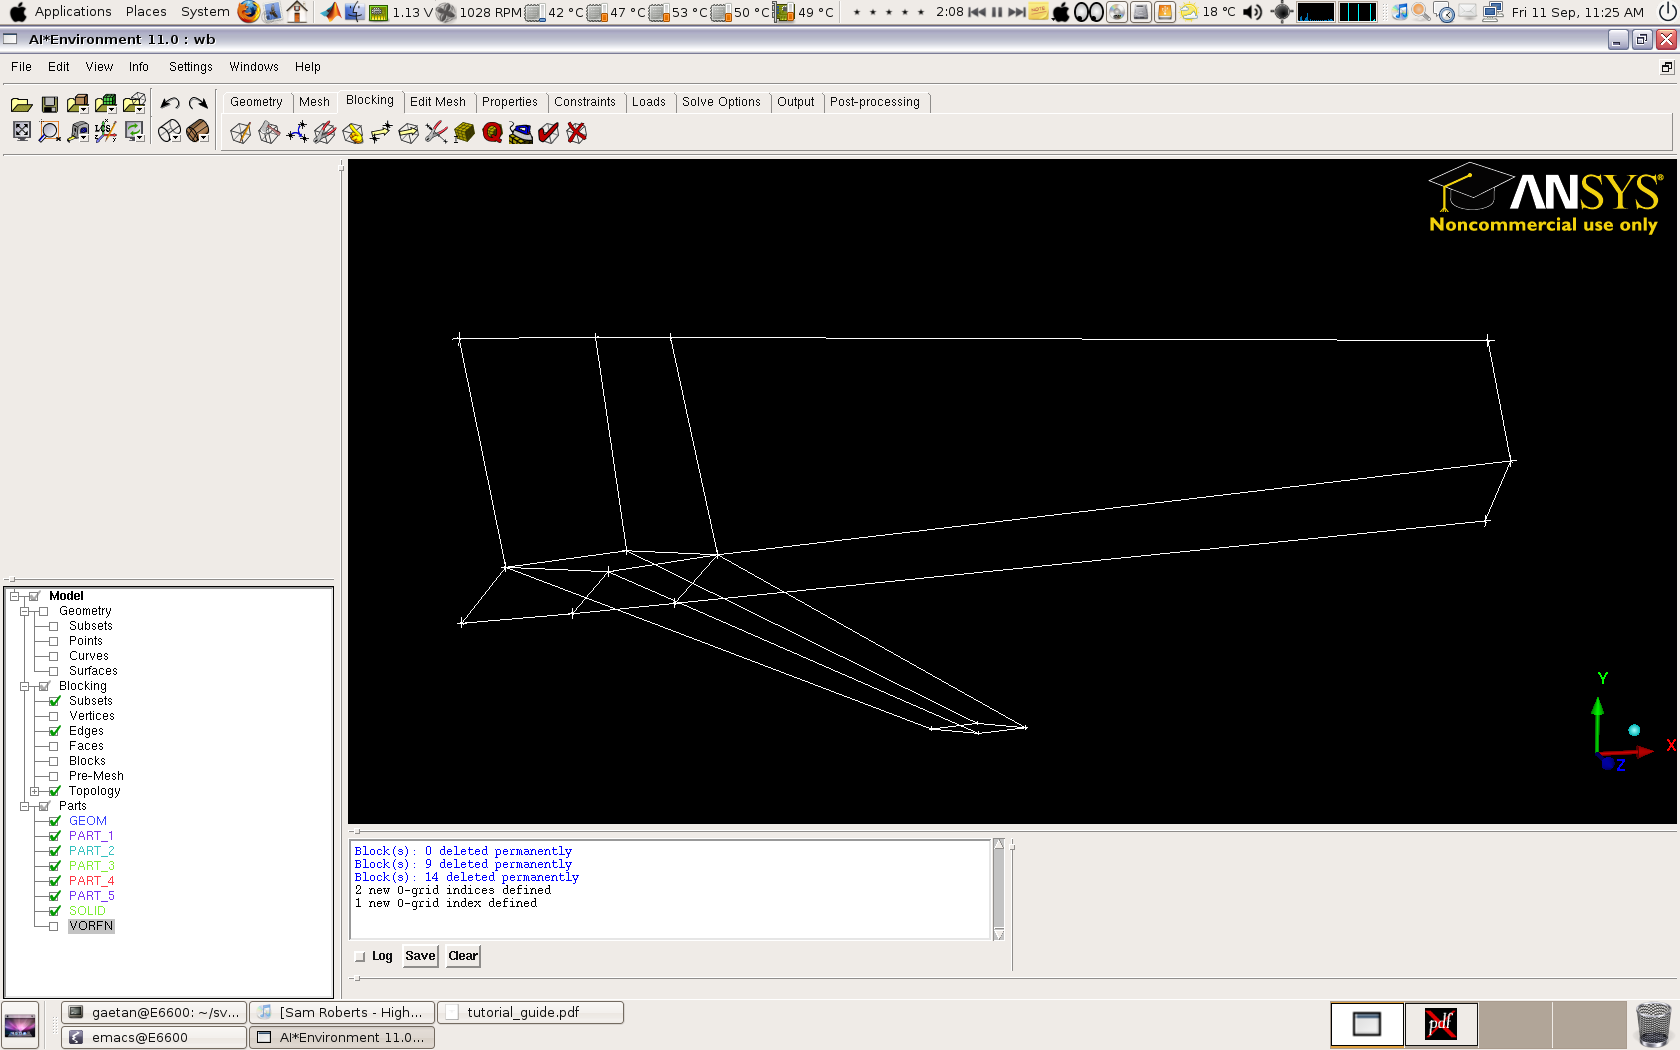
\includegraphics[width=\textwidth,angle=0]{figures/fig10.png}
  \caption{Fuselage and Wing Blocks}
  \label{fig:more_blocks}
\end{figure}

That takes care of the ``easy'' (non-degenerate blocks). The last blocks we must create are the two at the fuselage nose. Create them with 4 vertices. The two vertices towards the node, put one on the outer line and another on the curve we added previously as shown in figure~\ref{fig:nose_blocks}


\begin{figure}[htb]
  \centering
  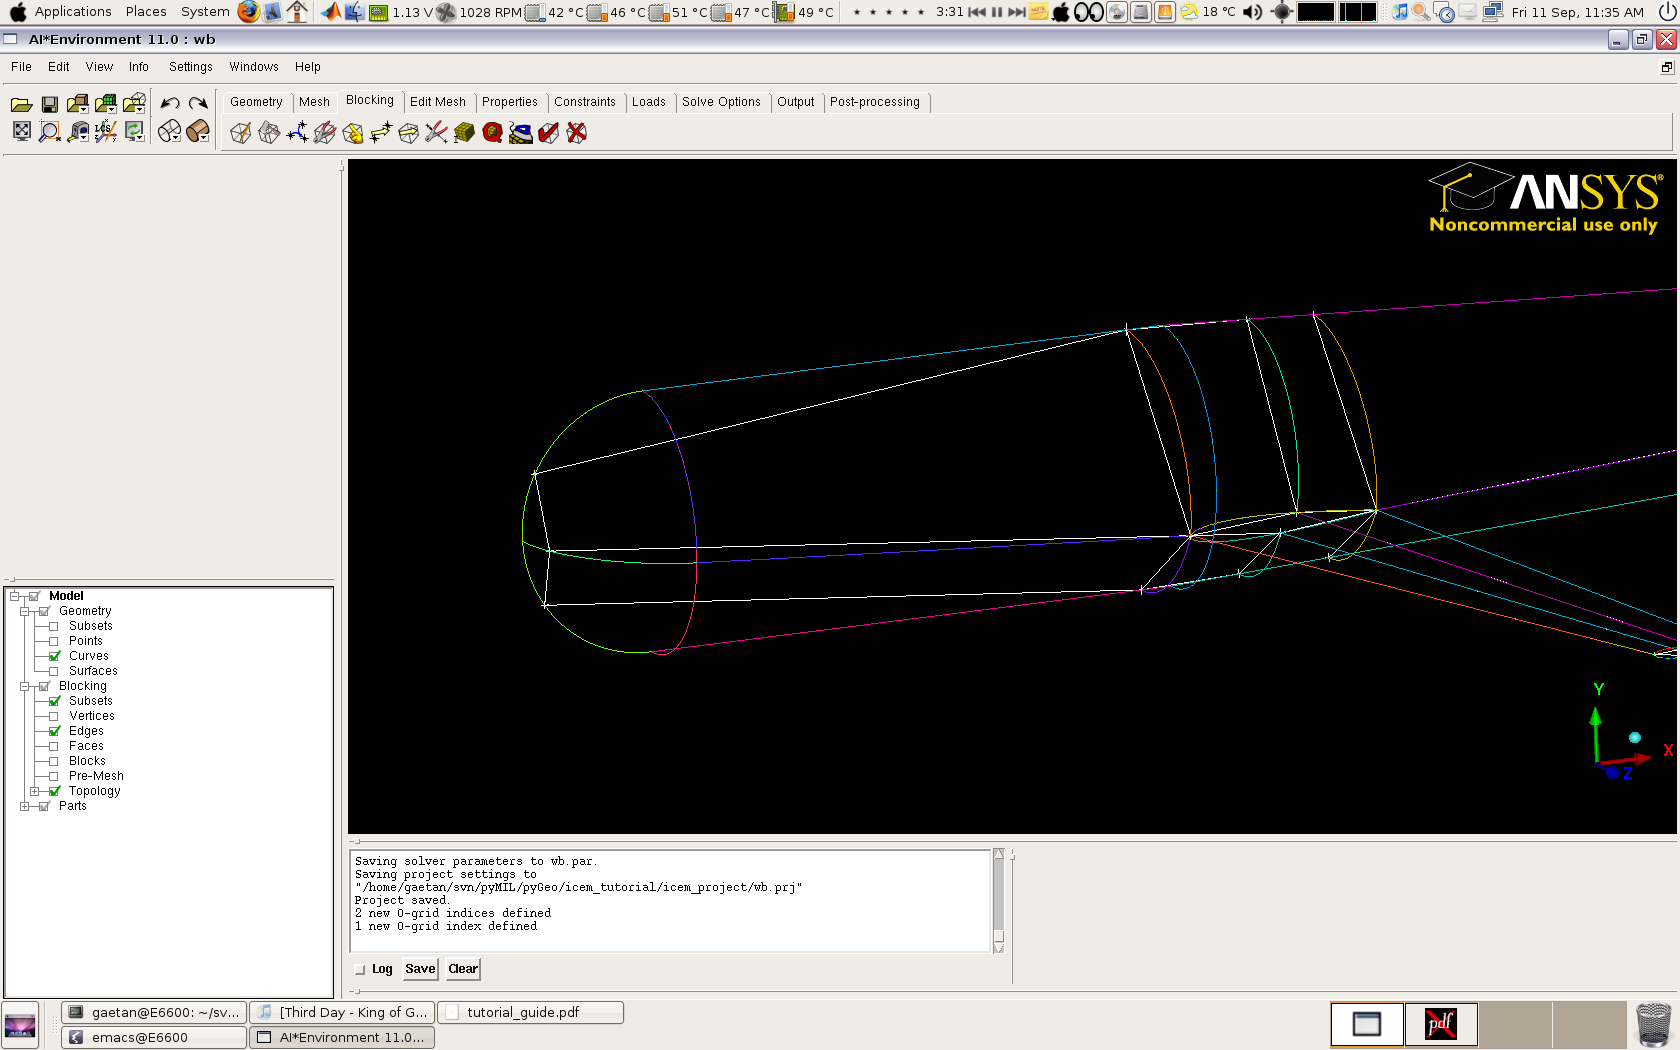
\includegraphics[width=\textwidth,angle=0]{figures/fig11.png}
  \caption{Nose Blocks}
  \label{fig:nose_blocks}
\end{figure}

A similar procedure can be done for the wing tip as well. Use the two vertices at the mid point the leading/trailing one and then create a dummy one on one of the other curves. This is shown in figure~\ref{fig:tip_blocks}

\begin{figure}[htb]
  \centering
  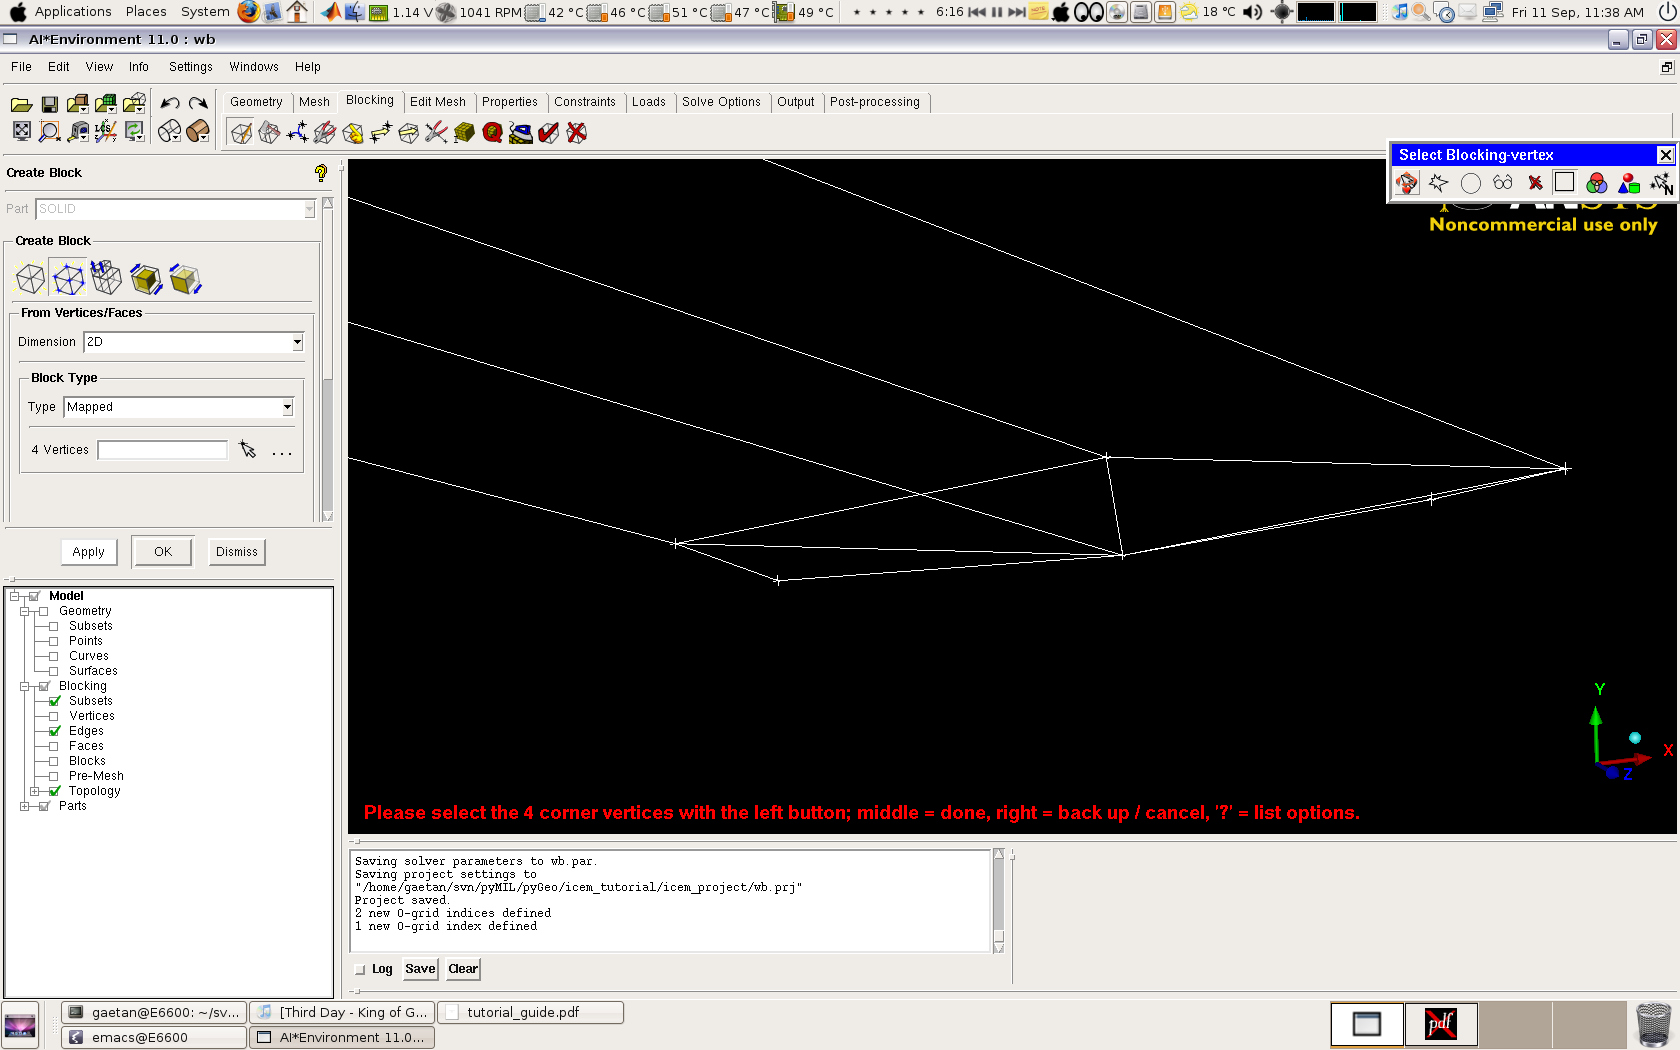
\includegraphics[width=\textwidth,angle=0]{figures/fig12.png}
  \caption{Tip Block detail. Note the ``extra'' node on the lower surface near the trailing edge and the extra one near the leading edge}
  \label{fig:tip_blocks}
\end{figure}

Now we will merge those extra edges to create a degenerate block.
Click the ``Merge Vertices'' button and use the first button ``Merge Vertices''. Leave the two vertices option selected and UNCLICK the propagate merge. THIS IS CRITICAL: DO NOT HAVE THE PROPAGATE MERGE BUTTON SELECTED. IT WILL NOT WORK! Figure~\ref{fig:nose_merged} shows the result of merging the vertices.

\begin{figure}[htb]
  \centering
  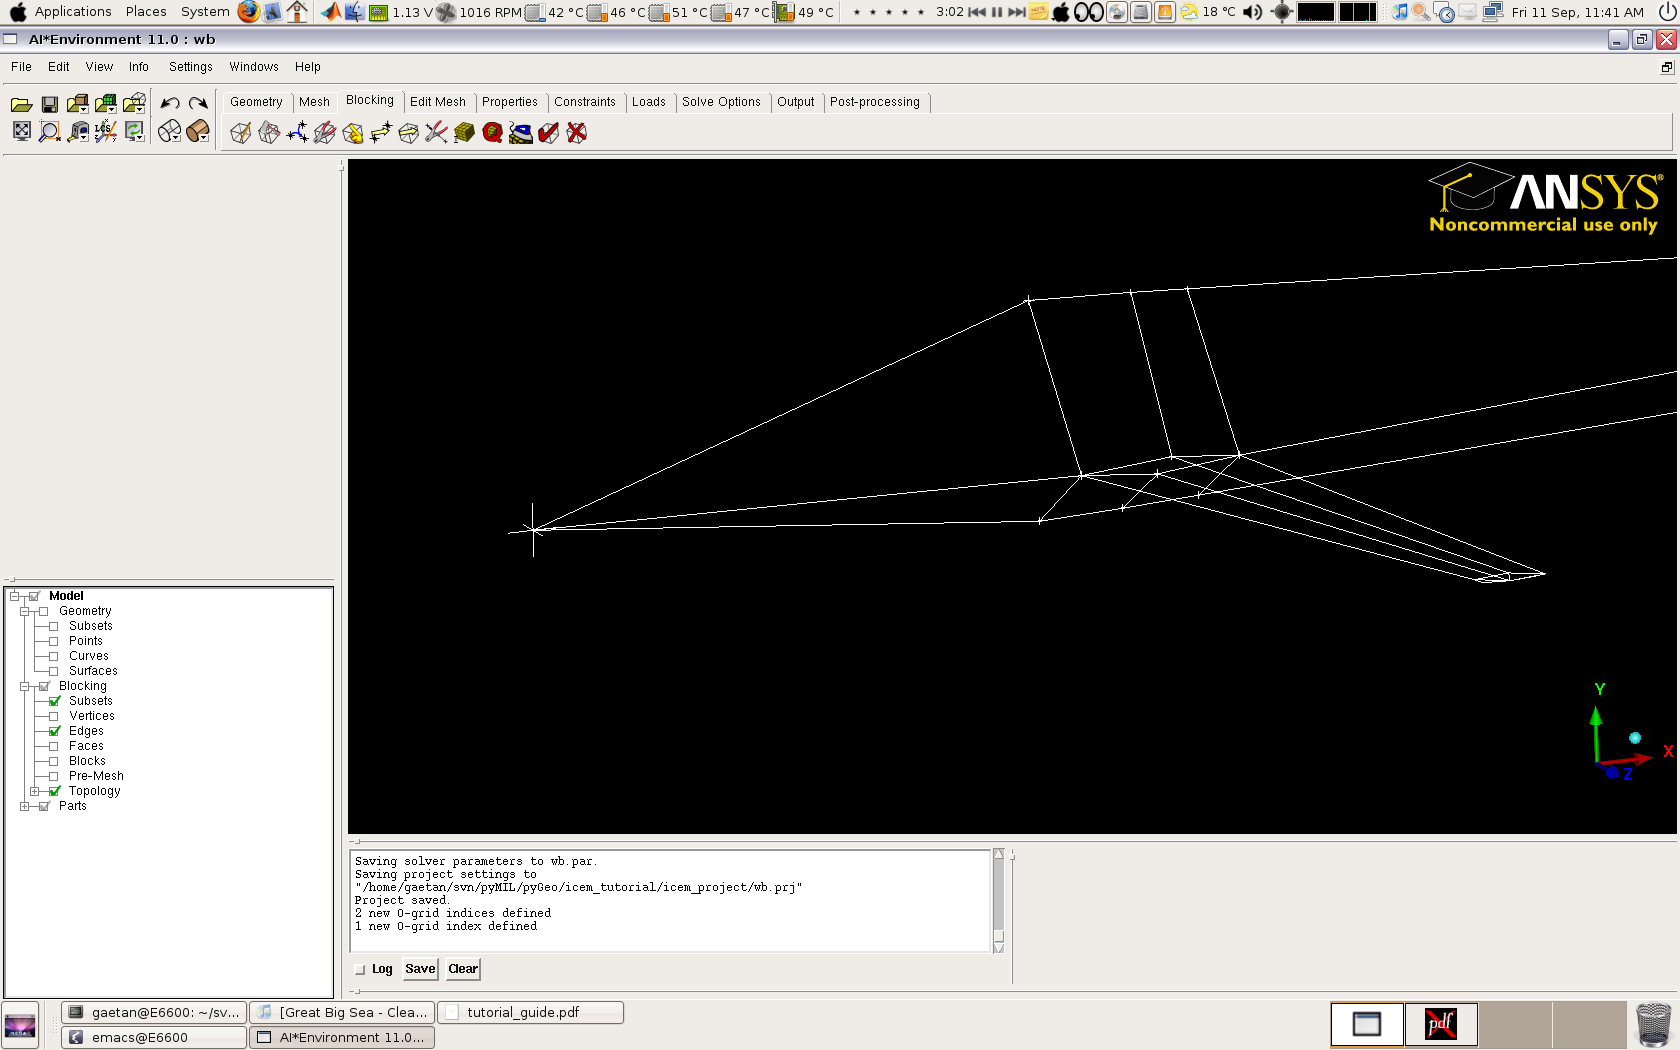
\includegraphics[width=\textwidth,angle=0]{figures/fig13.png}
  \caption{Vertices merged at leading edge}
  \label{fig:nose_merged}
\end{figure}

A similar procedure can be completed for the tip surfaces. 

Now, notice how all our edges are white, this means that are not associated with any physical geometry. This is the last step.

Click on the associate ``Associate'' button in the blocking tab. We first will associate ``edges'' to ``curves'' (Second Button). Now it should be clear why we made all those lines at the beginning; it is to associate the block edges to the geometry. For each edge, select the edge and its corresponding curve. 

Now notice (figure~\ref{fig:green_curves} how all the edges are green (except one on the tip which shouldn't matter).
\begin{figure}[htb]
  \centering
  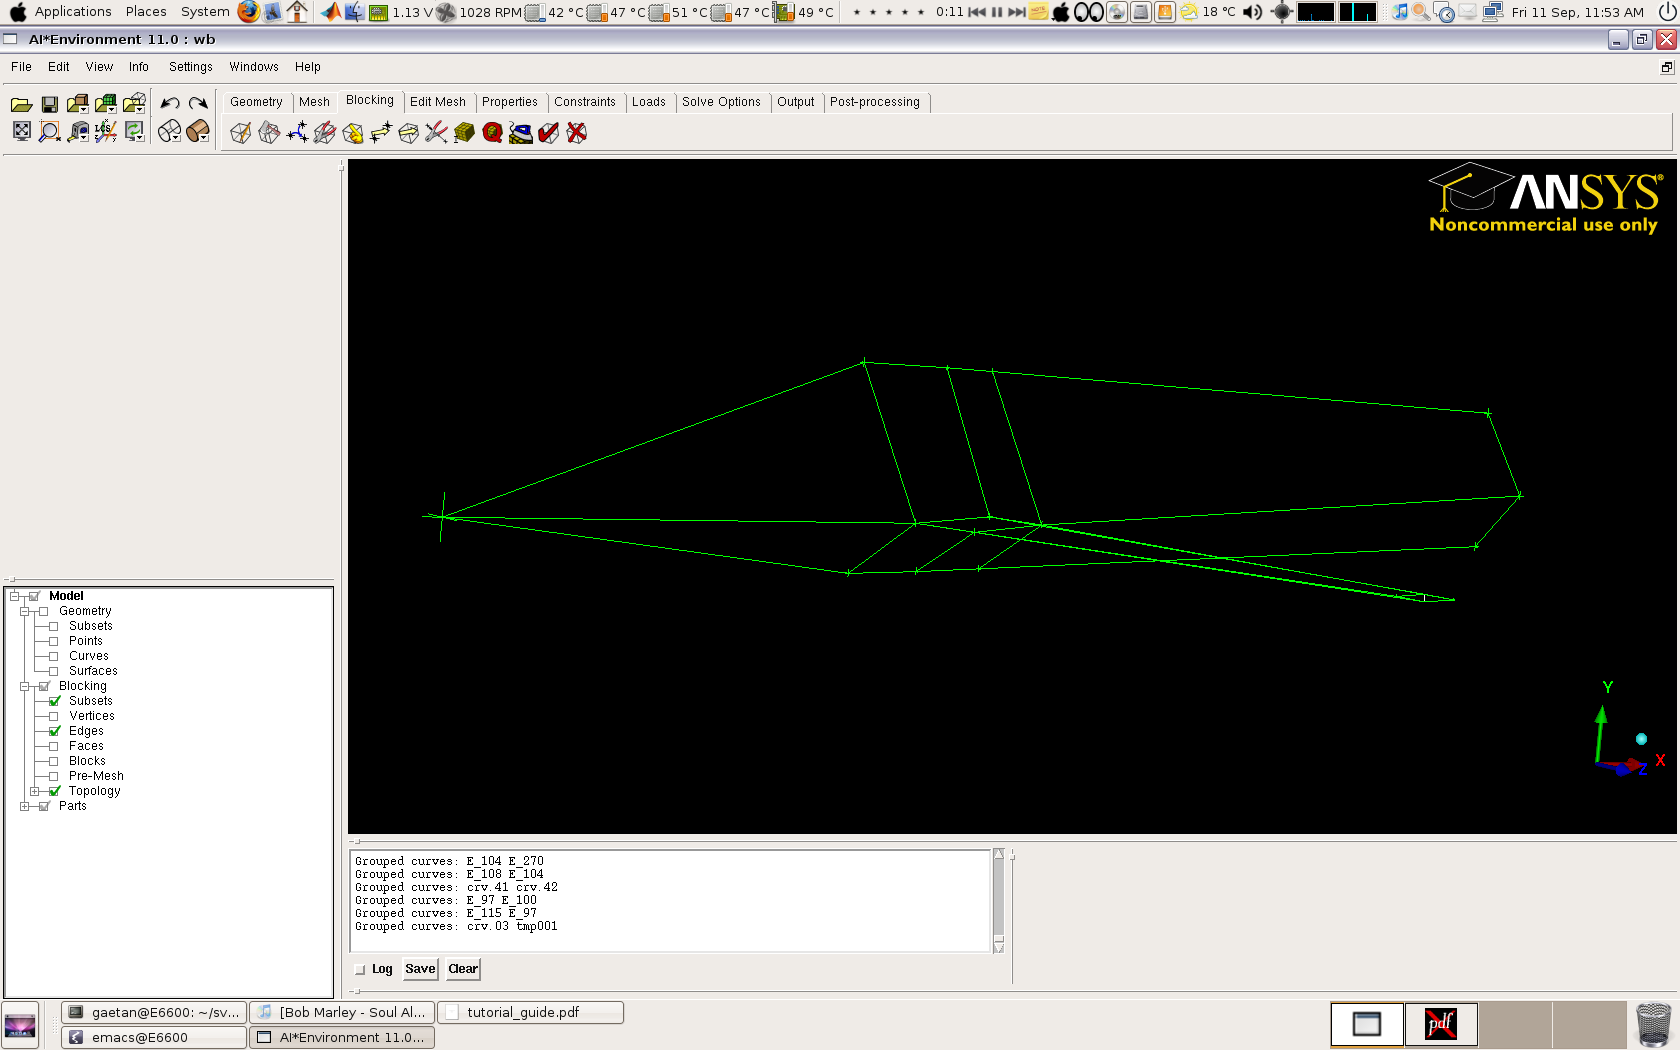
\includegraphics[width=\textwidth,angle=0]{figures/fig14.png}
  \caption{All vertices associated}
  \label{fig:green_curves}
\end{figure}

To make sure the curves are connected the way you think, right click on the edges and select ``Projected edge shape''. Turn off the geometry  curves (which will mask the edges). You should see something like figure~\ref{fig:projected_edge_shape}.
\begin{figure}[htb]
  \centering
  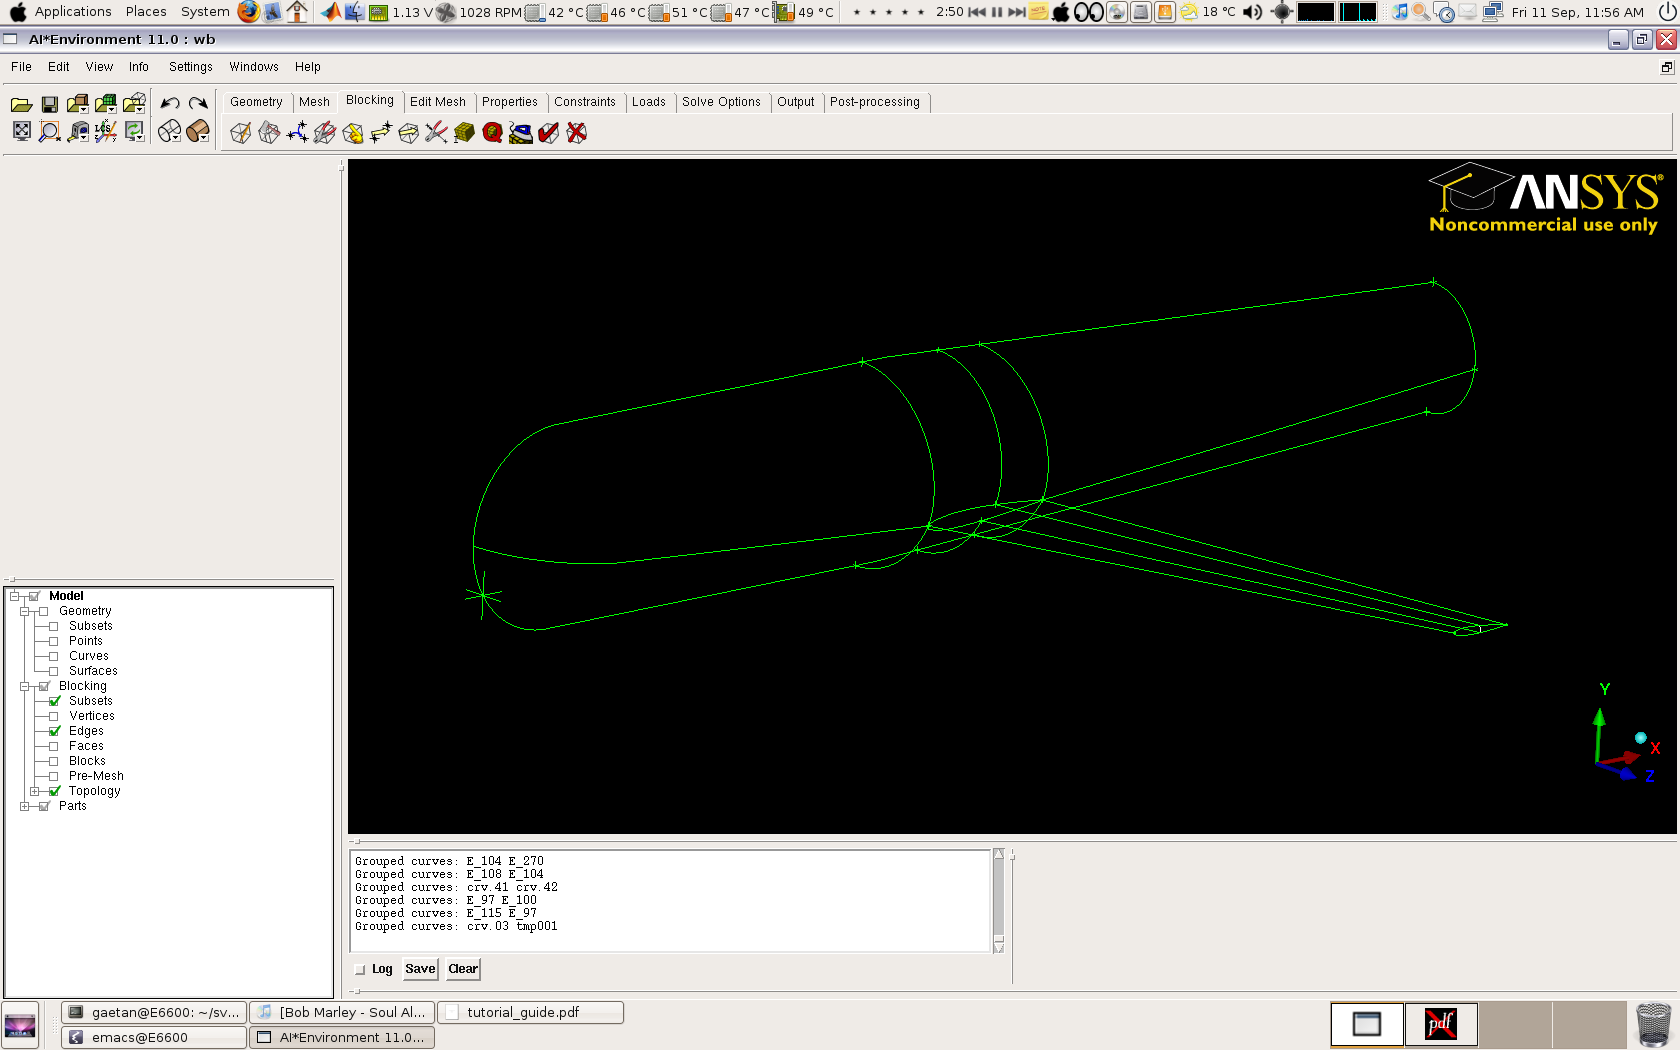
\includegraphics[width=\textwidth,angle=0]{figures/fig15.png}
  \caption{Projected Edge Shape}
  \label{fig:projected_edge_shape}
\end{figure}

The last thing we have to fix is the corner at the leading edge may not be exactly at the leading edge. Use the ``Associate Vertex'' command to associate the (degenerate) vertex at the leading edge with the point at the leading edge.

Now we can compute the mesh. Click on the ``Pre-Mesh'' option in the list on the left. It will probably ask to recompute the mesh. Select recompute. 

You probably wont' see a whole lot since the number of points on each edge is set to 2 by default. Click the ``Pre-mesh Params'' button under the blocking tab and click the third button ``Edge Params''. This lets you set the number of points on each edge. Select an edge and change the ``Nodes'' to something different. I put 10 in on every edge. This generated figure~\ref{fig:pre_mesh}.

\begin{figure}[htb]
  \centering
  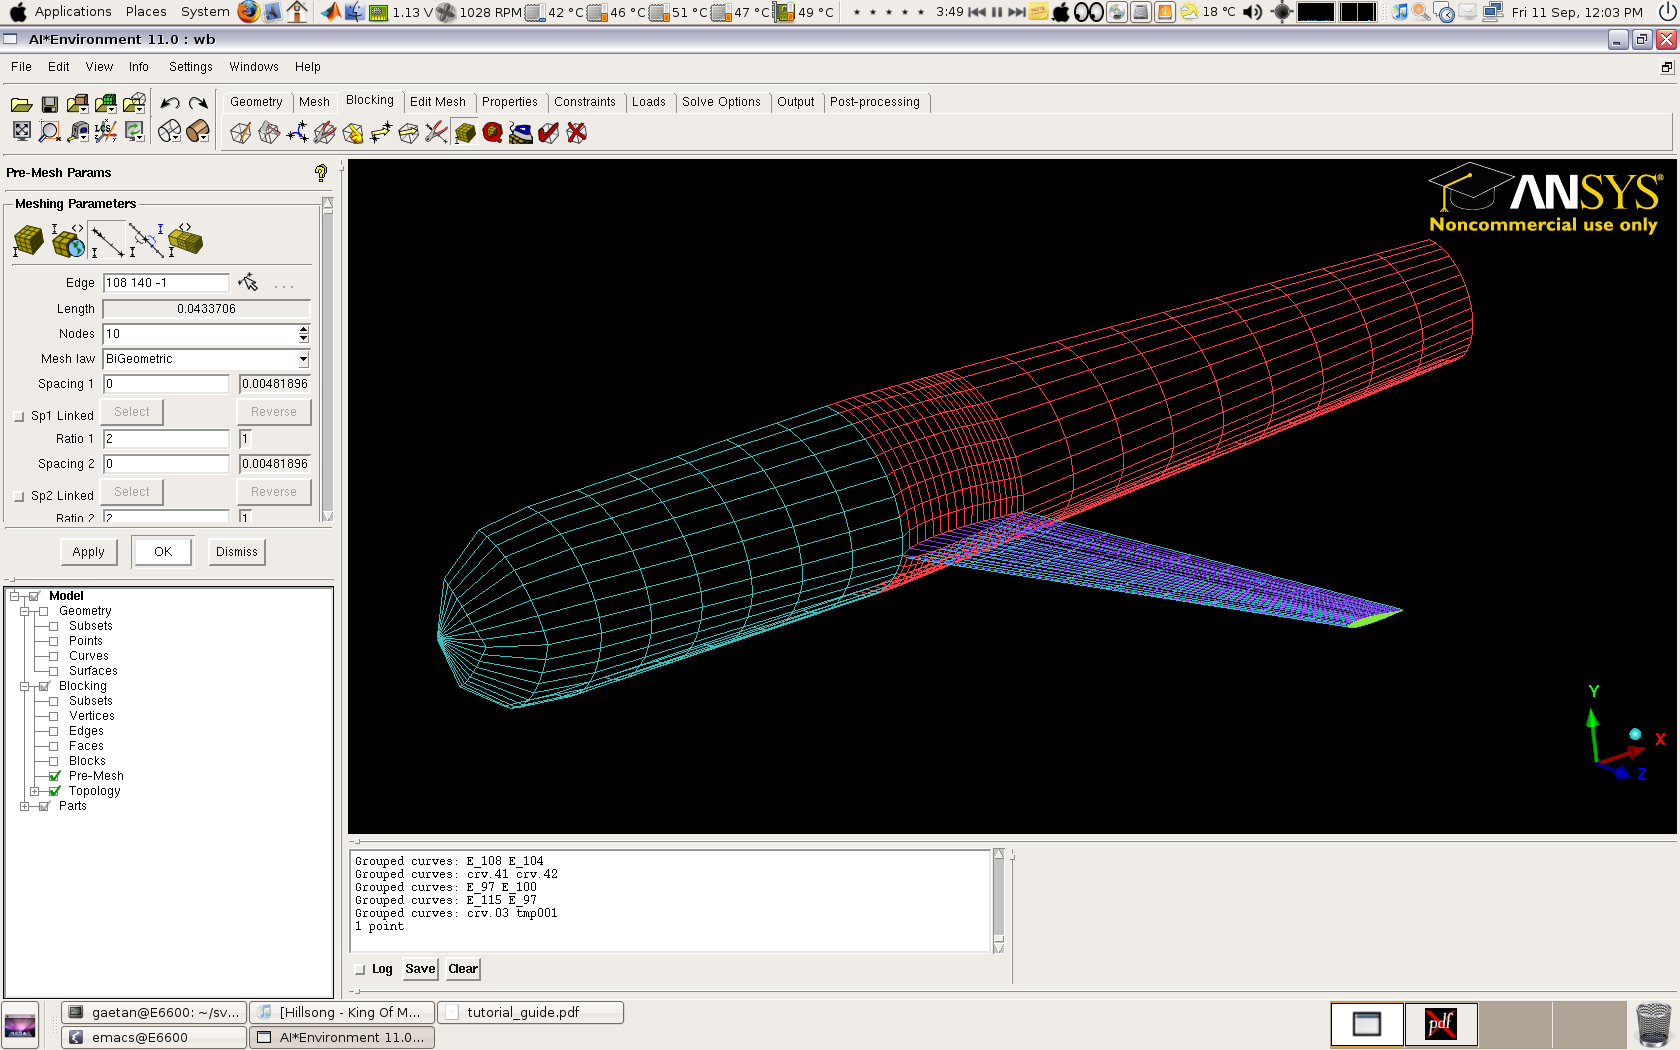
\includegraphics[width=\textwidth,angle=0]{figures/fig16.png}
  \caption{Computed Mesh}
  \label{fig:pre_mesh}
\end{figure}

It is now possible to experiment with the meshing density and type. Once the pre-mesh is acceptable, right click on ``Pre-Mesh'' on the left and click ``Convert to Multi-Block Mesh''.  This creates the actual mesh which will be exported.

\section{Output}

Once we have the multi-block surface mesh generated it can be exported by clicking on the ``Output'' tab. Then click the first button ``Select Solver'' and select ``Plot3D'' from the ``Output Solver'' list. Ignore the ``Common Structural Solver'' list. Click Ok.

Then click the last button, ``Write Input'' . It will ask to save the multiblock mesh, select the default. Finally you should get a plot3D output window show up as in figure~\ref{fig:plot3d_output}.

\begin{figure}[htb]
  \centering
  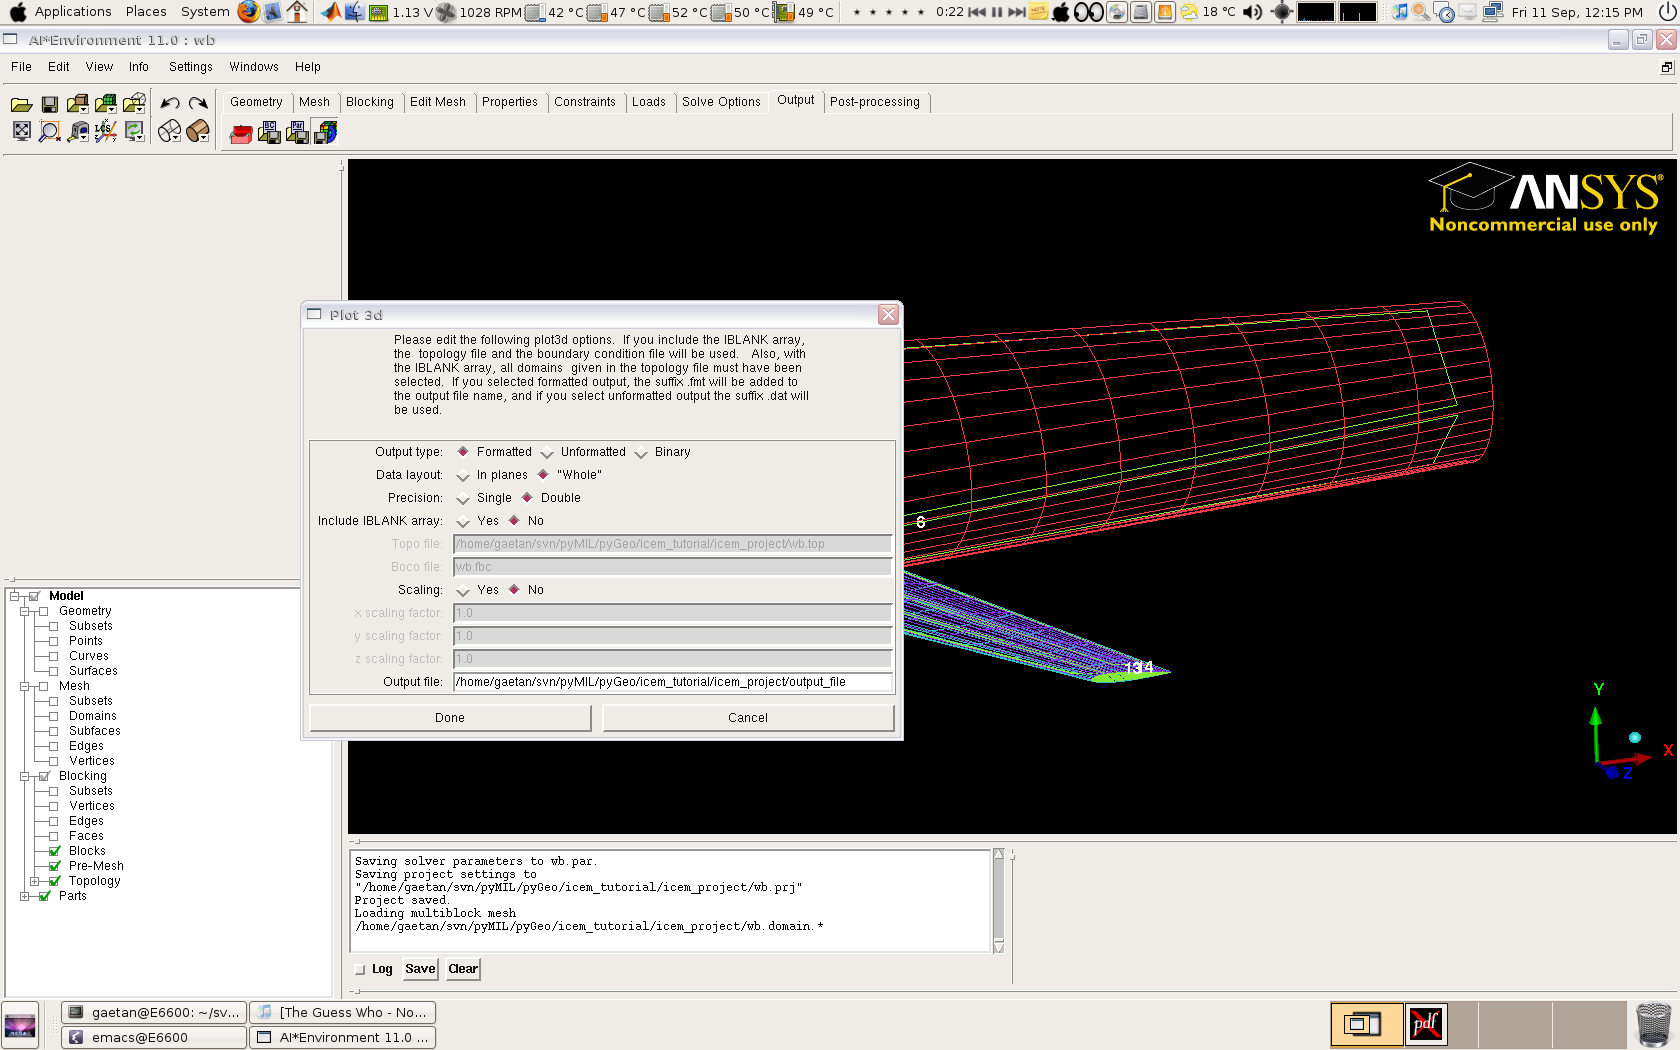
\includegraphics[width=\textwidth,angle=0]{figures/fig17.png}
  \caption{Plot3D Options}
  \label{fig:plot3d_output}
\end{figure}

Make sure the following options are used:
\begin{itemize}
\item Output Type: ``Formatted''
\item Data Layout: ``Whole''
\item Precision: ``Double''
\item Include IBLANK Array: ``No''
\item Scaling: ``No''
\item Output File: FILENAME
\end{itemize}

Now the output file, which will be called FILENAME.fmt can be read into pyGeo and the surfaces created from these blocked surface patches. 

\end{document}

%%% Local Variables:  %%% mode: latex %%% TeX-master: t %%% End: 